\documentclass[11pt,letterpaper]{article}
\usepackage[margin=0.9in]{geometry}
\usepackage[T1]{fontenc}
\usepackage{lmodern,microtype,amsmath,amssymb,booktabs,tabularx,graphicx}
\usepackage[dvipsnames]{xcolor}
\usepackage{listings,enumitem,tikz,fancyhdr,caption,float,needspace}
\usetikzlibrary{arrows.meta,positioning}
\usepackage[colorlinks=true,linkcolor=MidnightBlue,urlcolor=MidnightBlue,citecolor=MidnightBlue]{hyperref}
\definecolor{ink}{HTML}{243448}
\definecolor{accent}{HTML}{147E77}
\definecolor{codebg}{HTML}{F5F7F9}
\hypersetup{pdftitle={A Full 30-Round LLM Asset Market},pdfauthor={}}
\pagestyle{fancy}\fancyhf{}
\fancyhead[L]{\small EDSL full-market experiment}
\fancyhead[R]{\small GPT-5 mini / speculative-v1}
\fancyfoot[C]{\thepage}
\setlength{\headheight}{14pt}
\setlength{\parindent}{0pt}
\setlength{\parskip}{5pt}
\setlength{\emergencystretch}{2em}
\setlist{nosep,leftmargin=*}
\captionsetup{font=small,labelfont=bf}
\lstdefinestyle{python}{language=Python,basicstyle=\ttfamily\footnotesize,
 keywordstyle=\color{MidnightBlue}\bfseries,commentstyle=\color{OliveGreen},
 stringstyle=\color{BrickRed},backgroundcolor=\color{codebg},
 breaklines=true,breakatwhitespace=false,columns=fullflexible,keepspaces=true,
 showstringspaces=false,numbers=left,numberstyle=\tiny\color{gray},
 numbersep=7pt,xleftmargin=17pt,frame=single,framerule=0pt,
 aboveskip=9pt,belowskip=9pt,tabsize=4,
 literate={–}{{\textendash}}1}
\lstset{style=python}
\newcommand{\code}[1]{\texttt{\small #1}}
\newcommand{\source}[1]{\textit{Executed source:} \path{#1}. Line numbers refer to the frozen source file.}
\newcommand{\CodeSetup}{\lstinputlisting[firstline=1,lastline=47,firstnumber=1]{code/full_market_experiment.py}}
\newcommand{\CodePersonas}{\lstinputlisting[firstline=48,lastline=114,firstnumber=48]{code/full_market_experiment.py}}
\newcommand{\CodeQuestion}{\lstinputlisting[firstline=115,lastline=159,firstnumber=115]{code/full_market_experiment.py}}
\newcommand{\CodeMarket}{\lstinputlisting[firstline=160,lastline=200,firstnumber=160]{code/full_market_experiment.py}}
\newcommand{\CodePlan}{\lstinputlisting[firstline=201,lastline=220,firstnumber=201]{code/full_market_experiment.py}}
\newcommand{\CodeWorkflow}{\lstinputlisting[firstline=221,lastline=290,firstnumber=221]{code/full_market_experiment.py}}
\newcommand{\CodeRun}{\lstinputlisting[firstline=291,lastline=340,firstnumber=291]{code/full_market_experiment.py}}
\newcommand{\RuntimeBundle}{\lstinputlisting[firstline=1,lastline=126,firstnumber=1]{code/edsl/workflow_experiment.py}}
\newcommand{\RuntimeRun}{\lstinputlisting[firstline=127,lastline=257,firstnumber=127]{code/edsl/workflow_experiment.py}}
\newcommand{\RuntimeBatch}{\lstinputlisting[firstline=258,lastline=394,firstnumber=258]{code/edsl/workflow_experiment.py}}
\newcommand{\MarketDefinition}{\lstinputlisting[firstline=1,lastline=221,firstnumber=1]{code/edsl/call_market.py}}
\newcommand{\MarketAdmission}{\lstinputlisting[firstline=222,lastline=282,firstnumber=222]{code/edsl/call_market.py}}
\newcommand{\MarketSettlement}{\lstinputlisting[firstline=283,lastline=393,firstnumber=283]{code/edsl/call_market.py}}


\begin{document}
\begin{center}
{\LARGE\bfseries\color{ink} A Full 30-Round LLM Asset Market}\par
\vspace{5pt}
{\large Speculative traders, persistent state, and paired EDSL jobs}\par
{\small September 16, 2026 \quad $\cdot$ \quad One exploratory GPT-5 mini session}
\end{center}

\begin{abstract}
Twelve LLM traders completed a 30-round asset market with a constant \$14
fundamental value. Trading began at \$23.75 in round 5 and reached \$31 in
rounds 26--28, a 121.4\% premium to fundamental value. The market traded 114
shares across 21 rounds. There were no transactions in the last two rounds;
all 48 outstanding shares were then redeemed for \$14 under the announced
contract. Thus the run displays sustained overpricing and a rising price path,
but no observed market-price crash. EDSL elicited 360 fresh decisions; native
shared-state commands executed 30 settlements. Paired agent/scenario jobs
reduced full-round inference time to 30.5 seconds on average. This report
includes the complete experiment code, the workflow executor, and the native
market implementation. Economic mistakes in some responses remain an
important limitation despite a successful execution audit.
\end{abstract}

\section{Experiment and economic benchmark}
The design reconstructs the asset-market environment in the supplied
\emph{Building Traders} slides by Ngo et al.\ \cite{ngo}. It is not a numerical
replication of that study. Each trader starts with \$100 and four shares.
All 30 rounds were specified before this session began; there was no
price-based stopping rule. The earlier 17-round pilot is a separate market.
This session uses fresh answers, with the same seed and persona prompts.

After each round's trading, cash earns 5\% interest. Each share then pays the
same dividend, either \$0.40 or \$1.00 with equal probability. After round 30's
income, shares are redeemed for \$14. With $n=31-t$ payments remaining before
trading in round $t$, the expected present-value benchmark is
\[
 V_t=\sum_{k=1}^{n}\frac{0.70}{1.05^k}+\frac{14}{1.05^n}=14.
\]
This benchmark accounts for the return available on cash; simply adding
undiscounted future dividends to redemption overstates value. Monetary
operations in the implementation round to integer cents.

There are two traders of each type: Rational Arbitrageur (RA), Momentum
Chaser (MC), Bubble Timer (BT), Precommitter (PC), Noise Trader (NT), and
Overconfident Contrarian (OC). Seed 140926 fixes seats, dividend draws, and
equal-price priority. The newly authored \code{speculative-v1} prompts encourage
resale beliefs, early speculative interest, or exit plans, depending on type.
They are not the source authors' original prompts. The question states the
cash return, dividends, horizon, and redemption; it does not present the
\$14 valuation calculation or an opening market quote.

\clearpage
\section{Price formation and turnover}
\begin{figure}[H]
\centering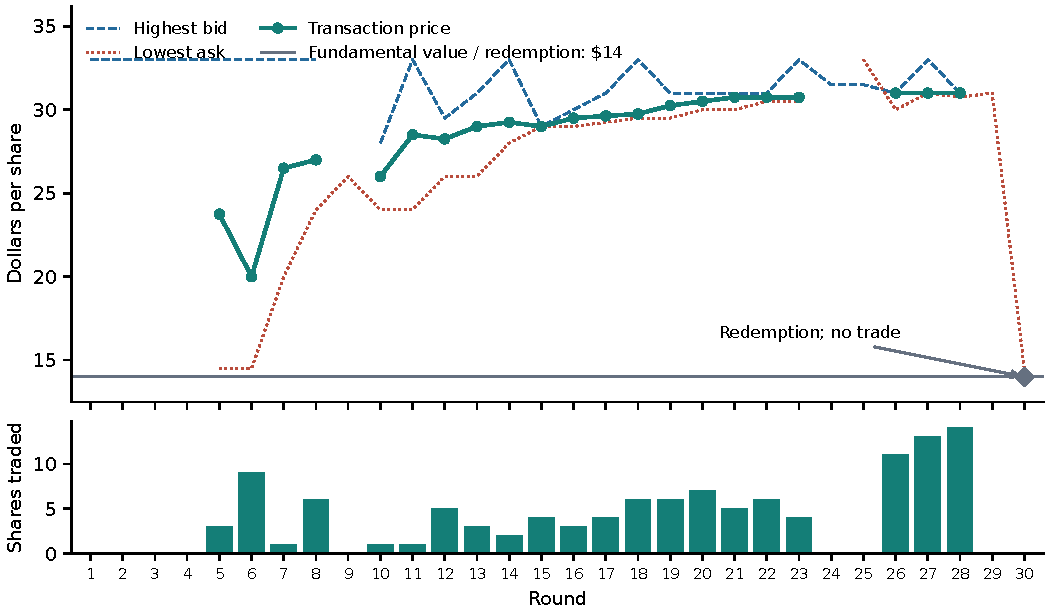
\includegraphics[width=\linewidth]{figures/prices.pdf}
\caption{Actual transaction prices, ex-post order-book summaries, and volume.
Gaps mean no trade. The diamond marks contractual redemption, not a transaction.
Traders saw the public transaction tape and their own histories, not the
other traders' sealed quotes shown here.}
\label{fig:prices}
\end{figure}

\begin{center}\small
\begin{tabular}{@{}lrrr@{}}
\toprule
Round(s) & Transaction price & Volume & Interpretation \\
\midrule
1--4 & --- & 0 & No trades \\
5 & \$23.75 & 3 & First transaction \\
6 & \$20.00 & 9 & Lowest observed price \\
26--28 & \$31.00 & 38 & Peak plateau \\
29--30 & --- & 0 & No final market trades \\
After round 30 & \$14.00 & --- & Redemption of 48 shares \\
\bottomrule
\end{tabular}
\end{center}

The first sale came from trader 09 (PC), who offered three initial shares at
\$14.50 according to its precommitted schedule. Trader 11 (OC) bought all three
with a \$33 limit. The uniform midpoint rule therefore produced
$(33+14.50)/2=\$23.75$. The first observed price was already 69.6\% above
fundamental value. Opening supply and a high bid jointly produced this result;
it does not show convergence from a market price near \$14.

Every observed transaction price exceeded fundamental value. From the first
trade to the peak, prices increased 30.5\%. Rounds 10--23 had fourteen consecutive
prices of at least \$17.50, although that diagnostic threshold did not stop the
run. Total turnover was 114 shares, or 2.375 times the outstanding stock of 48;
turnover counts repeated sales of the same shares. The volume-weighted price
was \$29.09. No post-peak decline was observed in transaction prices. The
redemption payment must not be plotted or described as a market crash.

\clearpage
\section{Every decision and fill}
\begin{figure}[H]
\centering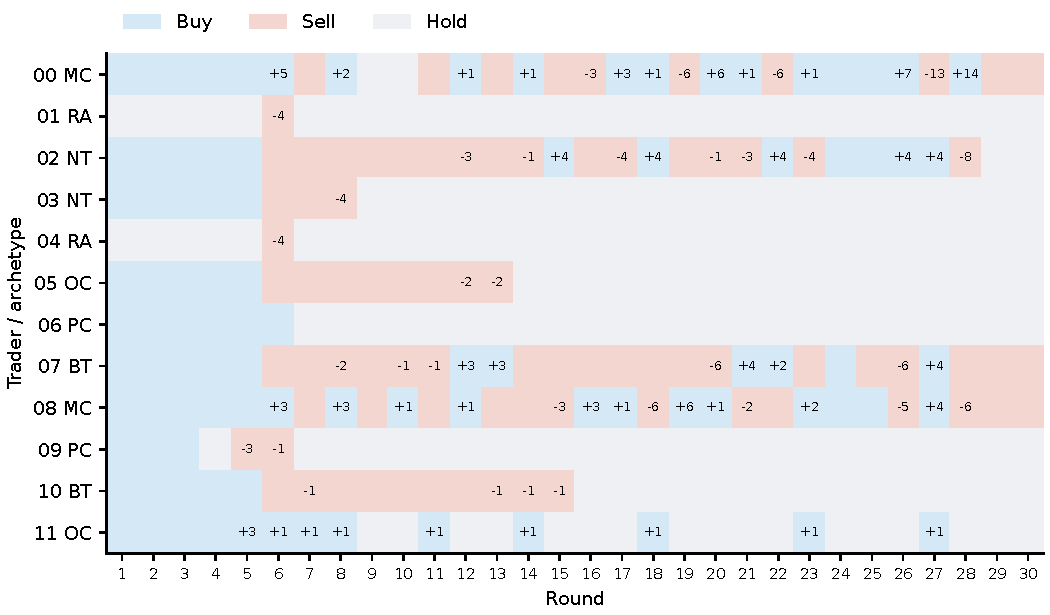
\includegraphics[width=\linewidth]{figures/decisions.pdf}
\caption{All 360 decisions. Cell color is the submitted side; numbers are
signed fills. A buy or sell without a number received no fill. The trader's
two-digit ID and archetype appear at left.}
\label{fig:decisions}
\end{figure}

There were 95 buy decisions, 83 sell decisions, and 182 holds. All orders passed
admission checks, and no requested quantities were reduced. Admission is not
execution: orders can be valid and still fail to cross another order.
The highest bid of \$33 in the early rounds was a quote, not a transaction.

Each trader submits a single sealed limit order: side, maximum buy price or
minimum sell price, and integer quantity. There is no borrowing or short
selling. Buys are capped by cash at the limit price and by 48 shares; sells
are capped by inventory. Orders expire after each round. The exchange requires
all twelve submissions, expands them into unit bids and asks, and sorts them
by price with a seeded tie lottery. If $b_k$ is the $k$th highest bid and $a_k$
the $k$th lowest ask, it executes the largest crossing quantity and uses one
price for all fills:
\[
 q=\max\{k:b_k\geq a_k\},\qquad
 p=\operatorname{round}_{\mathrm{cent}}\!\left(\frac{b_q+a_q}{2}\right).
\]
When no units cross, $q=0$ and the recorded transaction price is null.

Trading activity was concentrated. Trader 00 (MC) had 70 shares of gross
buy-plus-sell volume, trader 08 (MC) had 47, trader 02 (NT) had 44, and trader
07 (BT) had 32. These individual totals count both sides of an exchange;
market turnover counts each matched share once. Trader 06 (PC) never traded.
Some agents sold their initial four shares and then stayed out of the market.
This heterogeneity cautions against attributing a type-level effect to two
agents of each archetype in a single session.

\clearpage
\section{Final wealth and uncompleted exit plans}
\begin{figure}[H]
\centering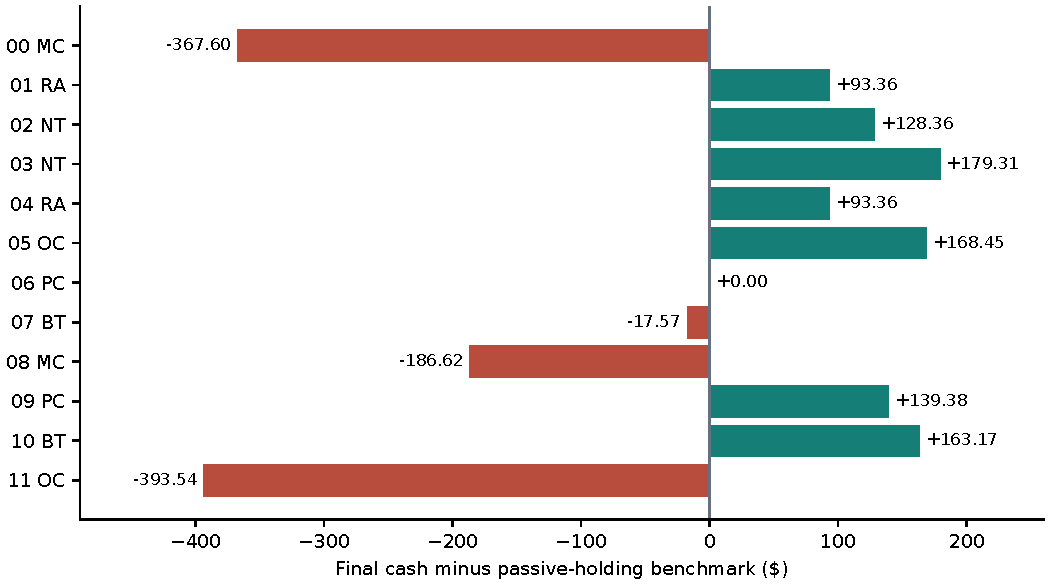
\includegraphics[width=\linewidth]{figures/wealth.pdf}
\caption{Final cash, including redemption, relative to holding \$100 and four
shares without trading. Applying the same realized dividends, interest order,
and cent rounding gives a passive final balance of \$648.69 per trader.}
\label{fig:wealth}
\end{figure}

Final cash ranged from \$255.15 (trader 11, OC) to \$828.00 (trader 03, NT).
Both rational arbitrageurs finished with \$742.05 after selling their four
initial shares in round 6. The passive precommitter, trader 06, finished with
exactly the \$648.69 benchmark. The two momentum chasers finished below that
benchmark: trader 00 with \$281.09 and trader 08 with \$462.07.

Near the end, trader 00 bought fourteen shares at \$31 in round 28. Its stated
rationale anticipated further price increases and later profit-taking.
Those fourteen shares alone cost \$434. There were no transactions in rounds
29--30, and trader 00 ultimately redeemed eighteen shares for \$252. Trader
11 redeemed fifteen shares and trader 08 redeemed seven. The remaining eight
shares were held by traders 06 and 07. All inventories became zero after
redemption; unrealized mark-to-market gains at the last \$31 trade were not
final cash profits.

The passive comparison holds the dividend path fixed and is an accounting
benchmark, not a causal estimate of the value of an archetype. Trading
redistributes wealth; per-account interest rounding leaves total realized cash
six cents above twelve passive accounts (\$7,784.34 versus \$7,784.28).
Appendix~\ref{app:wealth} gives every trader's terminal balance and inventory.

\clearpage
\section{What the responses do and do not establish}
The price series supports sustained speculative overpricing in this realized
session. It does not identify whether persona framing alone caused that
outcome, estimate a bubble frequency, or reproduce the source study's results.
There is one session, one model configuration, and no matched control here.
The prompts were deliberately written to encourage speculative behavior.
The midpoint exchange mechanism also directly shapes observed prices.

\subsection*{Economic and instruction-following errors}
The saved rationales reveal problems that a schema-valid answer does not rule
out. In round 5, trader 11 wrote:
\begin{quote}\small
``Fundamentals: remaining dividends $\approx$ 26 * \$0.7 = \$18.2 plus \$14
redemption $\to$ fair value $\approx$ \$32.2.''
\end{quote}
This calculation omits discounting at the available 5\% cash return. Its
\$33 bid enabled the first trade at \$23.75. This is evidence of a valuation
error in the elicited response, not proof of the model's internal reasoning
process. It complicates an interpretation based solely on intentional
resale speculation by a trader that fully understands fundamentals.

The prompt also explicitly requires forecasts beyond round 30 to equal the
\$14 redemption amount. Of 204 forecast entries with a beyond-terminal
horizon, nine failed that rule (4.4\%), across eight decisions and five traders.
Eight violations concerned the five-round horizon and one the two-round
horizon. For example, in round 28 trader 00 forecast \$35 five rounds ahead,
despite that horizon extending beyond the market's lifetime. It did give
\$14 at the ten-round horizon. The full prompts and answers for this decision
and the first buyer are included in the data bundle.

The execution audit checks that supplied information, accepted answers, and
state effects are consistent. It does not certify economic understanding.
The native forecast validator requires finite nonnegative numbers; it does
not enforce this terminal-horizon instruction. These violations were measured
afterward, not corrected during the run. A future controlled experiment could
separately manipulate comprehension checks, explicit valuation calculations,
persona wording, model choice, and clearing rules.

\subsection*{Model and execution record}
The configured model was \code{gpt-5-mini}, with temperature 1, medium reasoning,
and an 8,000-token completion allowance. EDSL called the hosted provider with
remote orchestration and caches disabled. ``Local'' execution here means the
EDSL runner ran locally; it does not mean an on-device language model. Recorded
model cost totaled \$1.2611. The seed fixes the market's random choices, not
fresh hosted-model responses.

\clearpage
\section{Workflow, batching, and validation}
\begin{figure}[H]
\centering
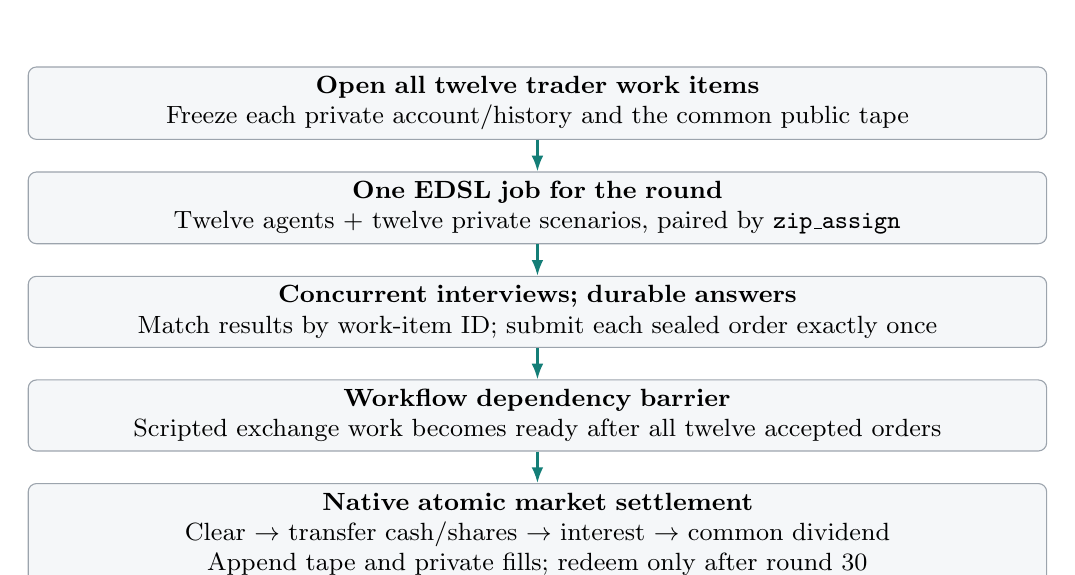
\begin{tikzpicture}[
 node distance=4mm,
 box/.style={draw=ink!45,rounded corners=3pt,fill=codebg,align=center,
 text width=12.7cm,minimum height=9mm,font=\small},
 arr/.style={-{Latex[length=2mm]},thick,draw=accent}]
\node[box] (s) {\textbf{Open all twelve trader work items}\\
 Freeze each private account/history and the common public tape};
\node[box,below=of s] (j) {\textbf{One EDSL job for the round}\\
 Twelve agents + twelve private scenarios, paired by \code{zip\_assign}};
\node[box,below=of j] (r) {\textbf{Concurrent interviews; durable answers}\\
 Match results by work-item ID; submit each sealed order exactly once};
\node[box,below=of r] (b) {\textbf{Workflow dependency barrier}\\
 Scripted exchange work becomes ready after all twelve accepted orders};
\node[box,below=of b] (e) {\textbf{Native atomic market settlement}\\
 Clear $\to$ transfer cash/shares $\to$ interest $\to$ common dividend\\
 Append tape and private fills; redeem only after round 30};
\foreach \a/\b in {s/j,j/r,r/b,b/e}{\draw[arr] (\a)--(\b);}
\end{tikzpicture}
\caption{The batched execution path. SQLite persists the workflow and market.
Each paired job is also saved as JSON.}
\end{figure}

\textbf{The batching change occurred during the run.} The first 140 decisions
ran serially. Execution stopped between completed calls, with no call in
flight, and resumed from the same saved specification and state. The four
remaining decisions in round 12 formed one job; rounds 13--30 each used one
12-interview job. No accepted answer was repeated. Paired assignments came
from PR \#2622, applied locally to the shared-state branch. Full batched jobs
averaged 30.5 seconds, compared with roughly 3--4 minutes per serial round.
This is an operational timing comparison, not a randomized speed benchmark.
The preserved prompts and information boundaries did not change.

The final audit found 360 unique trader calls, 360 order submissions, 30
settlements, and 390 successful workflow attempts. It reconstructed balances,
collateral constraints, fills, interest, dividends, all private read views,
rendered prompts, and final redemption of 48 shares. The batching change
passed 78 targeted tests and 287 broader regression tests; these are separate
runs with overlapping coverage, not 365 distinct tests. The authoring file
below matches the complete archived specification after normalization of
fresh internal identifiers. A full replay of all 360 saved answers through
the consolidated source reproduced the entire final market state, including
all histories, orders, balances, and redemption, without model calls.

\begin{thebibliography}{9}\small
\bibitem{ngo} Cady Ngo, Yi-Jhe Chen, Benjamin Manning, Christopher Avery, and
Colin Camerer. \emph{Building Traders: Persona Construction for LLM Agents in
Experimental Asset Markets}. Supplied 40-page presentation, \path{140926.pdf},
labelled September 18, 2026. Source checksum and page references are archived
in \path{data/source-paper.json}.
\bibitem{assignments} Expected Parrot. \emph{Add non-cartesian job assignments},
\href{https://github.com/expectedparrot/edsl/pull/2622}{PR \#2622}, head
\code{2077f01334cfc53460b119eb9927c3860c05ac4b}. Applied locally; this report
does not imply the PR was merged upstream.
\end{thebibliography}

\clearpage
\appendix
\section{Complete experiment source}\label{app:experiment}
This appendix reproduces \path{code/full_market_experiment.py} in full.
It is a post-run consolidation for readability, with no imports from another
experiment module. All personas, question text, economic parameters, workflow
steps, model settings, and execution commands are defined here. There is no
construction of an older pilot followed by survey replacement or removal of
pause rules. The complete definition was compared with the archived
\path{data/experiment.json}; only fresh UUIDs and the supplied creation timestamp
require normalization. The original executed builder and driver are separately
preserved under \path{code/historical/}.

The file depends on this branch's EDSL implementation and paired assignments
from PR \#2622. It is not a substitute for the full EDSL library. Appendices
B--C reproduce the relevant native executor and exchange implementation.

\subsection{Imports, constants, and answer schema}
Four forecast fields are followed by side, price, quantity, and rationale.
All quoted prices and forecasts are dollars; account balances are integer cents.
\CodeSetup

\subsection{Full persona instructions}
Each agent receives the common objective followed by exactly one of these
six persona strings. Each type appears twice in the shuffled population.
\CodePersonas

\subsection{Full question and private-history template}
The template includes the entire available private history and public tape.
The runtime resolves it before elicitation. It explicitly states the horizon,
interest/dividend ordering, and terminal redemption.
\CodeQuestion

\subsection{Agents and native economic rules}
The \code{call\_market} factory supplies the standard admission and settlement
commands. Income order and the marginal-midpoint price rule are explicit.
\CodeMarket

\subsection{The EDSL execution plan}
The exchange receives a literal scripted answer. That answer triggers the
settlement state command; no model performs the accounting.
\CodePlan

\subsection{All thirty rounds and the serializable bundle}
Every order step reads the session market and writes one order. Its settlement
step depends on all assigned traders. The next round depends on settlement.
There are no observation pause predicates in this construction.
\CodeWorkflow

\Needspace{7\baselineskip}
\subsection{Full command-line entry point}
Supplying \code{--responses} replays saved answers and prohibits fallback to
model calls. Omitting it launches paid hosted inference. Preparation alone
writes the definition without executing it. Resume reloads the pinned JSON.
\CodeRun

\clearpage
\section{Complete native workflow executor}\label{app:runtime}
The following is the complete \path{edsl/workflows/experiment.py} source used
for the batched continuation, copied to \path{code/edsl/workflow_experiment.py}.
It shows serialization and validation, durable launch/recovery, and the actual
EDSL job construction and execution. This is the updated implementation; the
initial serial implementation is identified by its hash in the original
source manifest. It is not silently represented as the batched version.

\subsection{Bundle, validation, and save/load}
The object contains workflow, states, agents, execution plan, and metadata.
Python callbacks and functional questions are rejected by this portable API;
standard capability implementations must be present in the installed runtime.
\RuntimeBundle

\subsection{Durable execution and recovery}
Work-item views are opened before answering any member of the ready batch.
Compatible LLM items are grouped by workflow step, model settings, and survey
schema. Scripted items and supplied replay responses bypass inference jobs.
\RuntimeRun

\subsection{One paired EDSL job per compatible batch}
Each participant gets its own scenario containing frozen question text and a
work-item ID. \code{zip\_assign(over=("agents", "scenarios"))} pairs row $i$
with row $i$, producing 12 interviews rather than a 144-interview cross-product.
Private text is not put into a scenario shared by all traders. Responses are
matched by ID and checked against the expected participant, independently of
completion order. Accepted submissions are retained if another result fails;
unfinished work is made retryable. Idempotency protects committed state
changes, not a blanket guarantee against repeated provider billing after a
network failure or crash.
\RuntimeBatch

\Needspace{0.24\textheight}
\section{Complete native call-market implementation}\label{app:market}
The source below is \path{edsl/sharedstate/call_market.py}, copied without
abbreviation. It defines the serialized rule parameters, private read view,
versioned commands, admission, and settlement. This is library code invoked by
the authoring file; it is not embedded Python inside the saved experiment JSON.

\subsection{Supported rules, machine construction, and private view}
The runtime validates policy choices before creating an execution database.
The view returns the requesting trader's account and public history, not the
full accounts map or the sealed order book. Unsupported versions or policies
fail explicitly.
\MarketDefinition

\subsection{Integer-cent conversion and sealed order admission}
Forecasts must be finite and nonnegative. This validation does not assess
valuation reasoning or enforce terminal-horizon forecast compliance.
\MarketAdmission

\subsection{Full clearing, income, and redemption logic}
The tie lottery and common dividend stream use distinct seed strings.
Settlement checks every trader has submitted, conserves cash and shares under
trading, applies the ordered income schedule, records fills, and redeems shares
only at the final round.
\MarketSettlement

\Needspace{0.30\textheight}
\section{Terminal accounts}\label{app:wealth}
Cash includes all realized income and terminal redemption. The final inventory
of every trader is zero. ``Redeemed'' records shares held immediately before
redemption. Difference is relative to passive final cash of \$648.69.

\begin{center}\small
\begin{tabular}{@{}llrrr@{}}
\toprule
Trader & Type & Final cash (\$) & Difference (\$) & Redeemed \\
\midrule
00 & MC & 281.09 & -367.60 & 18 \\
01 & RA & 742.05 & +93.36 & 0 \\
02 & NT & 777.05 & +128.36 & 0 \\
03 & NT & 828.00 & +179.31 & 0 \\
04 & RA & 742.05 & +93.36 & 0 \\
05 & OC & 817.14 & +168.45 & 0 \\
06 & PC & 648.69 & +0.00 & 4 \\
07 & BT & 631.12 & -17.57 & 4 \\
08 & MC & 462.07 & -186.62 & 7 \\
09 & PC & 788.07 & +139.38 & 0 \\
10 & BT & 811.86 & +163.17 & 0 \\
11 & OC & 255.15 & -393.54 & 15 \\
\bottomrule
\end{tabular}
\end{center}


\clearpage
\begingroup\small
\section{Reproduction and artifact guide}\label{app:reproduce}
\subsection{Replay the exact saved answers without model calls}
From the original repository root, replay through the complete consolidated
source below. This market has no pause rules, so one invocation executes all
30 rounds. Use a new output directory.
\begin{lstlisting}[language={},numbers=none]
python -m examples.asset_market.full_market_experiment \
  --responses examples/asset_market/full-market-note/data/responses.json \
  --output /private/tmp/full-market-source-replay-new
\end{lstlisting}
With only the report bundle, point \code{PYTHONPATH} at the updated EDSL
checkout and run \path{code/full_market_experiment.py} with the equivalent
paths. Installing an unrelated released EDSL version is insufficient.
A new model session omits \code{--responses}; its answers and prices need
not match this archive, even with the same seed.

\subsection{What is included}
\begin{center}\footnotesize
\begin{tabularx}{\linewidth}{@{}lX@{}}
\toprule
Path & Contents \\
\midrule
\path{report.pdf}, \path{report.tex} & Compiled report and editable LaTeX. \\
\path{code/} & Complete standalone experiment, audit/figure builders, native executor and market source, paired-assignment implementation, and historical builders. \\
\path{data/experiment.json} & Exact executed 30-round specification. \\
\path{data/responses.json} & All 360 answers for replay. \\
\path{data/market.json} & Final accounts, all histories, admitted orders, and tape. \\
\path{data/model-calls.jsonl.gz} & Compressed archive of all actual EDSL prompts and responses. \\
\path{data/round-13-job.json} & One complete saved 12-interview paired EDSL job. \\
\path{data/decisions.csv}, \path{data/periods.csv} & Decision/fill ledger and all 30 round outcomes. \\
\path{data/wealth-comparison.csv} & Final cash, passive benchmark, redeemed inventory. \\
\path{data/terminal-forecast-violations.csv} & All nine measured instruction violations. \\
\path{data/authoring-check.json}, \path{data/replay-check.json} & Specification comparison and complete saved-answer replay checks. \\
\path{data/batch-runner-transition.json} & Exact switchover record, PR revision, hashes, and test evidence. \\
\path{figures/}, \path{manifest.json} & Vector/PNG graphics and SHA-256 checksums. \\
\bottomrule
\end{tabularx}
\end{center}
The original SQLite databases and checkpoint backup remain in the repository's
run directory. The data in this bundle
can reproduce the state through replay; it does not duplicate those databases.
The source snapshots document the relevant code but are not a standalone EDSL
installation. Recorded source hashes distinguish the serial and batched
phases of the actual execution.

\subsection{Regenerate figures and compile}
The builder re-audits the saved run before copying artifacts or drawing figures.
It makes no model calls:
\begin{lstlisting}[language={},numbers=none]
python -m examples.asset_market.build_full_market_note
latexmk -cd -pdf -interaction=nonstopmode -halt-on-error \
  examples/asset_market/full-market-note/report.tex
\end{lstlisting}
A recipient of the bundle can compile \path{report.tex} directly: figures,
relative-path source listings, and generated tables are already included.
\endgroup

\end{document}
